\documentclass{article}
\usepackage[T2A]{fontenc}
\usepackage[utf8]{inputenc}
\usepackage[english,russian]{babel}
\usepackage{indentfirst}
\usepackage{amsfonts}
\usepackage{amsmath}
\usepackage{amsthm}
\usepackage{bbold}
\usepackage{moreverb}
\usepackage{dsfont}
\usepackage{graphicx}
\usepackage[colorlinks=true]{hyperref}

\DeclareMathOperator{\tr}{tr}
\DeclareMathOperator*{\argmin}{arg\,min}
\DeclareMathOperator*{\argmax}{arg\,max}
\newtheorem{theorem}{Теорема}


\title{Обучение с учителем. Дискриминантный анализ. Логистическая регрессия. Feature selection \& extraction.}
\author{Владимир Агеев, 622 гр.}
\date{\today}

\begin{document}
\maketitle
\tableofcontents
\section{Постановка задачи}
Обозначим $\boldsymbol{\xi} \in \mathbb{R}^p$ -- случайный вектор, вектор признаков, $\eta \in \mathcal{G} = \{G_k\}_{k = 1}^K$ -- дискретная случайная величина, отметка класса, $P(\boldsymbol{\xi}, \eta)$ -- их совместное распределение.

Пусть нам дана выборка $(\mathbf{x}_i, y_i)_{i = 1}^N$ -- $N$ реализаций случайных векторов $(\boldsymbol{\xi}, \eta)$. По выборке необходимо построить функцию $a: \mathbb{R}^p \rightarrow \mathcal{G}$, которая по реализации случайной величины $\boldsymbol{\xi}$ возвращает соответствующую метку класса $G \in \mathcal{G}$. В некотором смысле этот классификатор должен оказаться самым лучшим, минимально ошибаться.

Постановка задачи, в которой предполагается строить классификатор (или другую зависимость) исходя из данных ответов в выборке, называется обучением с учителем.

\section{Байесовский классификатор}

В качестве меры ошибки предсказания введем функцию потерь. Рассмотрим матрицу $\mathbf{L}$ размера $K \times K$, где $K = card(\mathcal{G})$. На диагонали $\mathbf{L}$ стоят нули, а $\mathbf{L}(i,j) = \lambda_{ij}$ -- цена ошибки отнесения элемента класса $G_i$ к классу $G_j$. Часто используется 0-1 функция потерь, где каждая ошибка оценивается единичкой.

Математическое ожидание функции потерь (средний риск):
\begin{align*}
  R(a) = \mathds{E}(\mathbf{L}(\eta, a(\boldsymbol{\xi}))) = \mathds{E}_{\boldsymbol{\xi}} \sum_{k = 1}^{K} L(G_k, a(\boldsymbol{\xi})) P(G_k \mid \boldsymbol{\xi}).
\end{align*}

Отсюда строим функцию классификации
\begin{align*}
  a(\mathbf{x}) = \argmin_{G \in \mathcal{G}} \sum_{k = 1}^{K} L(G_k, G) P(G_k \mid  \boldsymbol{\xi} = \mathbf{x}).
\end{align*}
Если подставим сюда 0-1 функцию потерь, получим
\begin{align*}
  a(\mathbf{x}) = \argmin_{G \in \mathcal{G}} 1 - P(G \mid \boldsymbol{\xi} = \mathbf{x}).
\end{align*}
Или, что то же самое
\begin{align*}
  a(\mathbf{x}) = \argmax_{G \in \mathcal{G}} P(G \mid \boldsymbol{\xi} = \mathbf{x}) = \argmax_{G \in \mathcal{G}} P(G)P(\boldsymbol{\xi} \mid \eta = G).
\end{align*}
Это решение называется байесовским классификатором, а такой подход -- принципом максимума апостериорной вероятности.

%Предположим, что $L(G, y) = \lambda_k$, если $k \neq y$ и $\lambda_k = 0$ иначе. Тогда функция потерь примет вид как в лекциях Воронцова
%\begin{align*}
  %a(x) = \argmax_{y \in G} \lambda_k P(y)P(x \mid G = y).
%\end{align*}

\section{Задача классификации на языке ML}\label{sec:MLClassification}
На языке ML рассмотрим задачу классификации. Пусть нам дана простая выборка $X^n = (x_i, y_i)_{i = 1}^n$, в которой наблюдения лежат в одном из двух классов $Y = \{-1, +1\}$.

Введем некотороые понятия:
\begin{itemize}
  \item $a(x, \beta) = \mathrm{sign}~f(x, \beta)$ -- семейство классификаторов;
  \item $M_i(\beta) = y_i f(x_i, \beta)$ -- отступ объекта $x_i$, мера принадлежности объекта $x_i$ классу $y_i$;
  \item $\mathcal{L}(M_i(\beta))$ -- монотонно невозрастающая функция потерь, мажорирующая 0-1 функцию потерь $[M < 0]$.
\end{itemize}
\bigskip
Задача поиска классификатора $a(x, \beta)$ сводится к задаче минимизации эмпирического риска
\begin{align*}
  Q(\beta, \mathbf{X}) = \sum_{i = 1}^N [M_i(\beta) < 0] \leq \sum_{i = 1}^N \mathcal{L}(M_i(\beta)) \rightarrow \min_\beta.
\end{align*}
Положив $\mathcal{L}(M_i(\theta)) = -\log P(x_i, y_i; \theta)$ получаем эквивалентность с задачей максимизации правдоподобия
\begin{align*}
  \sum_{i = 1}^N \log P(x_i, y_i; \theta) \rightarrow \max_\theta.
\end{align*}

\section{Дискриминантный анализ}

Для построения байесовского классификатора, нам необходимо знать апостериорные вероятности $P(G \mid \boldsymbol{\xi} = \mathbf{x})$. Обозначим $p_k(\mathbf{x}) = P(\boldsymbol{\xi} = \mathbf{x} \mid \eta = G_k)$ условные плотности классов, $\pi_k = P(\eta = G_k)$ -- априорные вероятности, $\sum_{k = 1}^{K} \pi_k = 1$. По теореме Байеса получим
\begin{align*}
   P(G = k \mid X = x) = \frac{p_k(x) \pi_k}{\sum_{i = 1}^K p_i(x)\pi_l}.
\end{align*}

Возникает вопрос: откуда брать априорные вероятности?
\begin{itemize}
  \item Брать равновероятные: $\pi_i = \frac{1}{K}$;
  \item Брать пропорционально объемам классов $\pi_i = \frac{n_i}{N}$;
  \item Соответственно имеющейся информации. Например, исходя из цены ошибки классификации.
\end{itemize}

\subsection{Квадратичный дискриминантный анализ}
Предположим, что каждый класс имеет многомерное нормальное распределение $P(\boldsymbol{\xi} \mid \eta = G_k) = \mathcal{N}_p(\mu_k, \mathbf{\Sigma}_k)$, его плотность
\begin{align*}
  p_k(\mathbf{x}) = \frac{1}{(2\pi)^{p/2} \lvert \mathbf{\Sigma}_k \rvert^{1/2}} e^{-\frac{1}{2}(\mathbf{x} - \mu_k)^\mathrm{T} \mathbf{\Sigma}_k^{-1}(\mathbf{x} - \mu_k)}.
\end{align*}
Подставим плотности в байесовский классификатор, который мы получили в предыдущем пункте и получим
\begin{multline*}
  a(\mathbf{x}) = \argmax_{i \in 1 \ldots K} \pi_i p_i(\mathbf{x}) = \argmax_{i \in 1 \ldots K} \log(\pi_i p_i(\mathbf{x}))
  = \argmax_{i \in 1 \ldots K} \log(\pi_i) + \log(p_i(\mathbf{x})) = \\
  = \argmax_{i \in 1 \ldots K}(-\frac{1}{2}(\mathbf{x} - \mu_i)^\mathrm{T} \mathbf{\Sigma}_i^{-1}(\mathbf{x} - \mu_i) - \frac{1}{2}\log(\lvert \mathbf{\Sigma}_i \rvert) + \log(\pi_i)) = \argmax_{i \in 1 \ldots K} g_i(\mathbf{x}).
\end{multline*}
Заметим, что получившийся классификатор квадратично зависит от $\mathbf{x}$, отсюда название quadratic discriminant analysis.

\subsection{Линейный дискриминантный анализ}
Предположим теперь, что классы имеют нормальное распределение с одинаковой ковариационной матрицей, то есть $P(\boldsymbol{\xi} \mid \eta = G_k) = \mathcal{N}_p(\mu_k, \Sigma)$. Отсюда следует, что классификатор, полученный в предыдущем пункте, можно упростить следующим образом:
\begin{multline*}
  a(\mathbf{x})
  = \argmax_{i \in 1 \ldots K}(-\frac{1}{2}(\mathbf{x} - \mu_i)^\mathrm{T} \mathbf{\Sigma}^{-1}(\mathbf{x} - \mu_i) - \frac{1}{2}\log(\lvert \mathbf{\Sigma} \rvert) + \log(\pi_i)) = \\
  = \argmax_{i \in 1 \ldots K}(-\frac{1}{2} \mu_i^\mathrm{T} \mathbf{\Sigma}^{-1}\mu_i + \mu_i^\mathrm{T} \mathbf{\Sigma}^{-1}x + \log(\pi_i)) =  \argmax_{i \in 1 \ldots K} \delta_i(x).
\end{multline*}
Такой классификатор зависит от $\mathbf{x}$ линейно.

Разделяющая два класса гиперплоскость определяется так
\begin{multline*}
  \{\mathbf{x} : \delta_i(\mathbf{x}) = \delta_j(\mathbf{x})\} =\\ = \{x : -\frac{1}{2} (\mu_i - \mu_j)^\mathrm{T} \mathbf{\Sigma}^{-1}(\mu_i + \mu_j) + (\mu_i - \mu_j)^\mathrm{T} \mathbf{\Sigma}^{-1}\mathbf{x} + \log(\pi_i/\pi_j) = 0\}.
\end{multline*}
От соотношения между априорными вероятностями зависит положение границы относительно классов (к какому она ближе).

%\subsection{Геометрический смысл линейного дискриминанта}
%В одномерной проекции на направляющий вектор разделяющей гиперплоскости классы разделяются наилучшим образом, то есть с минимальной ошибкой.

\subsection{Оценка параметров}
На практике параметры распределений классов нам не известны, поэтому предлагается использовать следующие оценки максимального правдоподобия параметров нормальных плотностей классов.
\begin{itemize}
  \item Среднее
  $\widehat{\mu}_i = \frac{1}{n_i}\sum\limits_{j: y_j = G_i} \mathbf{x}_j$,
  \item Ковариационная матрица класса $\widehat{\mathbf{\Sigma}}_i = \frac{1}{n_i - 1}\sum\limits_{j: y_j = G_i} (\mathbf{x}_j - \widehat{\mu}_i)^\mathrm{T}(\mathbf{x}_j - \widehat{\mu}_i)$,
  \item Pooled ковариационная матрица $\widehat{\mathbf{\Sigma}}= \sum\limits_{j = 1}^K\frac{n_i - 1}{n - K} \widehat{\mathbf{\Sigma}}_i$.
\end{itemize}

\subsection{Возвращение к вероятностям}
Если нам необходимо получить вероятности отношения $\mathbf{x}$ к классу $i$, то, вычислив $\widehat{\delta}_i(\mathbf{x})$, можно вычислить
\begin{align*}
  \widehat{P}(\eta = G_i \mid \boldsymbol{\xi} = \mathbf{x}) = \frac{e^{\widehat{\delta}_i(\mathbf{x})}}{\sum\limits_{j = 1}^K e^{\widehat{\delta}_j(\mathbf{x})}}.
\end{align*}

\subsection{Regularized Discriminant Analysis}
Оценка ковариационной матрицы $\widehat{\mathbf{\Sigma}}_i$ может оказаться выражденной или плохо обусловленной. Опишем компромис между LDA и QDA, а так же борьбу с мультиколлинеарностью.
\begin{itemize}
  \item Regularized Discriminant Analysis. Рассматривается матрица $\widehat{\mathbf{\Sigma}}_i(\alpha) = \alpha \widehat{\mathbf{\Sigma}}_i + (1 - \alpha)\widehat{\mathbf{\Sigma}}$, где $\widehat{\mathbf{\Sigma}}$ -- pooled ковариационая матрица. Здесь $\alpha \in [0, 1]$ порождает континуум моделей между LDA и QDA, выбирается скользящим контролем.
  \item Дополнительно к предыдущему методу можно похожим образом модифицировать pooled ковариационную матрицу и рассматривать $\widehat{\Sigma}(\gamma) = \gamma \widehat{\mathbf{\Sigma}} + (1 - \gamma)\sigma^2 \mathbf{I}_p$, где $\gamma$ определяет вид ковариационной матрицы и выбирается скользящим контролем.
\end{itemize}

\subsection{Наивный байесовский классификатор}
Предположим, что признаки независимы внутри групп и имеют нормальное распределение
  \begin{align*}
    p_i(x) = \prod_{j = 1}^p p_{ij}(x_j), \quad p_{ij}(x_j) = \frac{1}{\sqrt{2\pi}\sigma_{ij}}e^{-\frac{(x_j - \mu_{ij})^2}{2\sigma^2_{ij}}}.
  \end{align*}
  Отсюда классифицирующую функцию можно представить в виде
  \begin{align*}
    \delta_i(x) = -\frac{1}{2}\sum_{j = 1}^p\frac{(x_j - \mu_{ij})^2}{2\sigma^2_{ij}} + \log(\pi_i).
  \end{align*}

Аналогично подходам выше, можно подбирать ковариационную матрицу скользящим контролем в виде
\begin{align*}
  \widehat{\mathbf{\Sigma}}_i(\alpha) = \alpha \widehat{\mathbf{\Sigma}}_i + (1 - \alpha)~\mathrm{diag}(\sigma^2_{i1}, \ldots, \sigma^2_{ip}).
\end{align*}

Такой подход может быть полезен, когда признаков очень много и оценивать плотности классов оказывается сложно. Плотности $p_{ki}$ можно оценивать по отдельности, а если признак дискретный, для этого можно использовать гистограмму.

Не смотря на такое оптимистичное предположение, наивный Байес часто превосходит более сложные методы.

%\subsection{Вычисление дискриминантной функции}
%Рассмотрим следующие шаги
%\begin{itemize}
  %\item $\widehat{\mathbf{\Sigma}}_k = \mathbf{U}_k \mathbf{D}_k \mathbf{U}_k^\mathrm{T}$ -- спектральное разложение;
  %\item $(\mathbf{x} - \mu_k)^\mathrm{T} \mathbf{\Sigma}_k^{-1}(\mathbf{x} - \mu_k) = [\mathbf{U}_k^\mathrm{T}(\mathbf{x} - \mu_k)]^\mathrm{T} \mathbf{D}_k^{-1}[\mathbf{U}_k^\mathrm{T}(\mathbf{x} - \mu_k)]$;
  %\item $\log |\widehat{\mathbf{\Sigma}}_k| = \sum_l \log d_{kl}$.
%\end{itemize}


\subsection{Уменьшение размерности}
К feature extraction в традиционном дискриминантном анализе подходят следующим образом.

Задача: найти линейное преобразование $\mathbf{Z} = A^\mathrm{T}\mathbf{X}$, в результате которого получаются признаки наилучшим образом разделяющие группы.  Хотелось бы, чтобы эти признаки оказались ортогональны. Далее опишем эту задачу более формально.

\begin{itemize}
  \item $\widehat{\mathbf{\Sigma}} = \mathbf{U} \mathbf{D} \mathbf{U}^\mathrm{T}$, -- pooled ковариационная матрица
  \item $\mathbf{X}^\ast = \mathbf{D}^{-\frac{1}{2}}\mathbf{U}^\mathrm{T} \mathbf{X}$ -- нормировали матрицу данных относительно pooled ковариационной матрицы
  \item Перейдем от матрицы данных $\mathbf{X}^\ast$ к матрице центров групп $\mathbf{M}_{K, p}$
  \item Вычислим внутриклассовую ковариационную матрицу
  \begin{align*}
        \mathbf{W} = \frac{1}{n - K} \sum\limits_{i = 1}^K \sum_{j: y_j = G_i} (\mathbf{x}_j - \widehat{\mu}_i)^\mathrm{T}(\mathbf{x}_j - \widehat{\mu}_i)
  \end{align*}
  \item Вычисляем межклассовую ковариационную матрицу (с точностью до коэффициента)
  \begin{align*}
        \mathbf{B} = \sum\limits_{i = 1}^K n_i (\widehat{\mu}_i - \widehat{\mu})^\mathrm{T}(\widehat{\mu}_i - \widehat{\mu}).
  \end{align*}
\end{itemize}

Пусть $\zeta = A\boldsymbol{\xi}$ -- новый признак, тогда распределение $P(\zeta \mid \eta = G_k) = \mathcal{N}_p(A^\mathrm{T}\mu_k, A^\mathrm{T}\mathbf{\Sigma}_kA)$.

На выборочном языке новые признаки $Z =A^\mathrm{T}\mathbf{X}$. Выборочная ковариационная матрица (с точностью до коэффициента) новых признаков имеет вид
\begin{align*}
A^\mathrm{T}\mathbf{T}A = A^\mathrm{T}(\mathbf{W} + \mathbf{B})A = A^\mathrm{T}\mathbf{W}A + A^\mathrm{T}\mathbf{B}A,
\end{align*}
где $\mathbf{T}$ -- total covariance matrix, первое слагаемое -- оценка внутригрупповых отклонений, а второе -- оценка межгрупповых отклонений. Воспользовавшись критерием Фишера перейдем к обобщенной задаче на собственные числа и собственные вектора:
\begin{align*}
  \frac{A^\mathrm{T}\mathbf{B}A}{A^\mathrm{T}\mathbf{W}A} \rightarrow \max_{A}.
\end{align*}

Путь $\lambda_1 \geq \lambda_2 \geq \ldots \geq \lambda_d$ -- собственные числа матрицы $\mathbf{W}^{-1}\mathbf{B}$, а $A_1, \ldots, A_d$ -- соответствующие им собственные вектора. Тогда максимум выше равен $\lambda_1$  и достигается на $A_1$. При этом $A^\mathrm{T}_i \mathbf{W}A_j = 0$. Далее
\begin{align*}
  \max_{A, A \bot A_1}\frac{A^\mathrm{T}\mathbf{B}A}{A^\mathrm{T}\mathbf{W}A} = \lambda_2,
\end{align*}
достигается на $A_2$ и так далее.

Вектора $A_i$ называют каноническими коэффициентами, а новые признаки $Z_i$ -- каноническими переменными, $Z_i$ ортогональны в обычном смысле.

%\begin{figure}
%  \includegraphics[width=\linewidth]{variance.pdf}
  %\caption{A boat.}
%  \label{fig:boat1}
%\end{figure}


\subsection{Значимость канонических переменных}
Возникает вопрос: сколько канонических переменных нам окажется достаточно взять? Другими словами, нужно проверить гипотезу
\begin{align*}
  H_0: A_i, i = \ell,\ldots,d~\text{не описывают отличия}.
\end{align*}
Введем статистику $\Lambda-prime$:
\begin{align*}
\Lambda_\ell^p = \prod_{i = l}^d \frac{1}{1 + \lambda_i}.
\end{align*}
Тогда гипотезу выше можно переформулировать так
\begin{align*}
H_0: \Lambda_\ell^p = 1 \Leftrightarrow \lambda_\ell = \ldots = \lambda_d = 0 \Leftrightarrow rank \mathbf{B} = \ell - 1.
\end{align*}

Критерий:
\begin{align*}
t = \Lambda_{\ell}^{p} \sim \Lambda_{\nu_\mathbf{B} + (\ell - 1), \nu_\mathbf{W} - (\ell - 1)}.
\end{align*}

\subsection{Последовательный дискриминантный анализ}
Опишем подход к feature selection в дискриминантном анализе на обычном языке.

Возникает вопрос отбора признаков. С одной стороны нам бы хотелось, чтобы признаки были независимы, с другой -- убрать признаки, которые не влияют на качество разделения. Для начала более формально определим от каких признаков мы хотим избавиться:
\begin{itemize}
  \item Признаки, которые являются линейной комбинацией других признаков, другими словами имеют большой коэффициент множественной корреляции $\mathbf{R}^2 = \mathbf{R}^2(\xi_i;\{\xi_j \mid j \neq i\})$ (по pooled ковариационной матрице);
  \item Признаки, которые не влияют на качество разделения. Действуем аналогично пошаговой регрессии. Введем статистику
  \begin{multline*}
    (Partial \Lambda)_i = \Lambda(X_i \mid X_1, \ldots, X_{i - 1}, X_{i + 1}, \ldots, X_p) = \\
    = \frac{\Lambda(X_1, \ldots, X_p)}{\Lambda(X_i \mid X_1, \ldots, X_{i - 1}, X_{i + 1}, \ldots, X_p)} = \frac{1}{1 + \lambda_i}.
  \end{multline*}
  Гипотеза:
  \begin{align*}
    H_0 :~\text{добавление  $X_i$ не влияет на качество разделения} \Leftrightarrow (Partial \Lambda)_i = 1.
  \end{align*}
  Критерий (принимая во внимание соотношение между распределением $\Lambda_1(\nu_\mathbf{B}, \nu_\mathbf{W} - p + 1)$ и распределением Фишера):
  \begin{align*}
    F_i = \frac{1 - (Partial \Lambda)_i / \nu_\mathbf{B}}{(Partial \Lambda)_i/ (\nu_\mathbf{W} - p + 1)} \sim F_{\nu_\mathbf{B}}.
  \end{align*}
  Далее жадным образом отбираем признаки, влияющие на качество разделения.
\end{itemize}

\subsection{LDA как минимизация эмпирического риска}
В данном разделе сведем задачу максимизации апостериорных вероятностей к задаче минимизации эмпирического риска.

Покажем, что задача максимизации эмпирического риска эквивалентна решению обобщенной задачи на собственные числа. Обобщенная задача на собственные вектора имеет вид
\begin{align*}
    \mathbf{B}A = \lambda\mathbf{W}A.
\end{align*}
Заметим, что матрицу $\mathbf{W}$ можно заменить на ковариационную матрицу $\mathbf{\Sigma}$ так как она является суммой $\mathbf{B}$ и  $\mathbf{W}$ и такая замена не изменит собственные вектора. В случае двух групп одинакового размера
\begin{align*}
\sum_{i = 1}^2 m (\mathbf{\mu}_i - \frac{\mathbf{\mu}_1 + \mathbf{\mu}_2}{2})(\mathbf{\mu}_i - \frac{\mathbf{\mu}_1 + \mathbf{\mu}_2}{2})^\mathrm{T}A = \lambda \mathbf{\Sigma}A.
\end{align*}
Далее
\begin{align*}
 m(\mathbf{\mu}_1 - \mathbf{\mu}_2)(\mathbf{\mu_1} - \mathbf{\mu}_2)^\mathrm{T}A = \lambda \mathbf{\Sigma}A.
\end{align*}
В левой части стоит ортогональный проектор на прямую $\langle (\mu_1 - \mu_2) \rangle$. Следовательно, с точностью до константы (которую мы можем <<вложить>> в собственное число)
\begin{align*}
  \lambda\mathbf{\Sigma}A = (\mathbf{\mu}_1 - \mathbf{\mu}_2), \quad A \propto \mathbf{\Sigma}^{-1}(\mathbf{\mu}_1 - \mathbf{\mu}_2).
\end{align*}
Полученный вектор является вектором нормали к разделяющей гиперплоскости и совпадает с тем, что мы получаем в байесовском подходе.

Известно, что LDA в форме обобщенной задачи на собственные вектора эквивалентен каноническому корреляционному анализу \footnote{См. доказательство например \href{https://www.stat.washington.edu/wxs/Stat592-w2011/Slides/cancorr-notes.pdf}{здесь}}. С другой стороны CCA в случае, когда одна из групп признаков одномерная, совпадает с линейной регрессией.

Таким образом, LDA эквивалентно линейной регрессии вида
\begin{align*}
  \sum_{i = 1}^N\left(\mathbf{x}^\mathrm{T}_i\mathbf{\beta} + \beta_0-y_i\right)^2 \rightarrow \min\limits_{\mathbf{\beta},\beta_0}.
\end{align*}
Как и выше, мы предполагаем, что представителей классов ${-1, 1}$ поровну, т.е. $\sum_{i = 1}^N y_i = 0$ и априорные вероятности в LDA равны. Такая задача эквивалентна
\begin{align*}
  \sum_{i = 1}^N\left((\mathbf{x}^\mathrm{T}_i\mathbf{\alpha} + \alpha_0)y_i - 1\right)^2 \rightarrow \min\limits_{\mathbf{\alpha},\alpha_0},
\end{align*}
где $\mathbf{\alpha}$ и $\mathbf{\alpha}_0$ отличаются от $\mathbf{\beta}$ и $\mathbf{\beta}_0$ только масштабом. Полученная задача и есть ERM.

Задача максимизации апостериорных вероятностей эквивалентна минимизации аппроксимации эмпирического риска (см. Рис. \ref{fig:quadraticLoss})
\begin{align*}
  Q(\alpha, \alpha_0) = (1 - M(\alpha, \alpha_0))^2.
\end{align*}



\begin{figure}[h]

  \begin{center}
  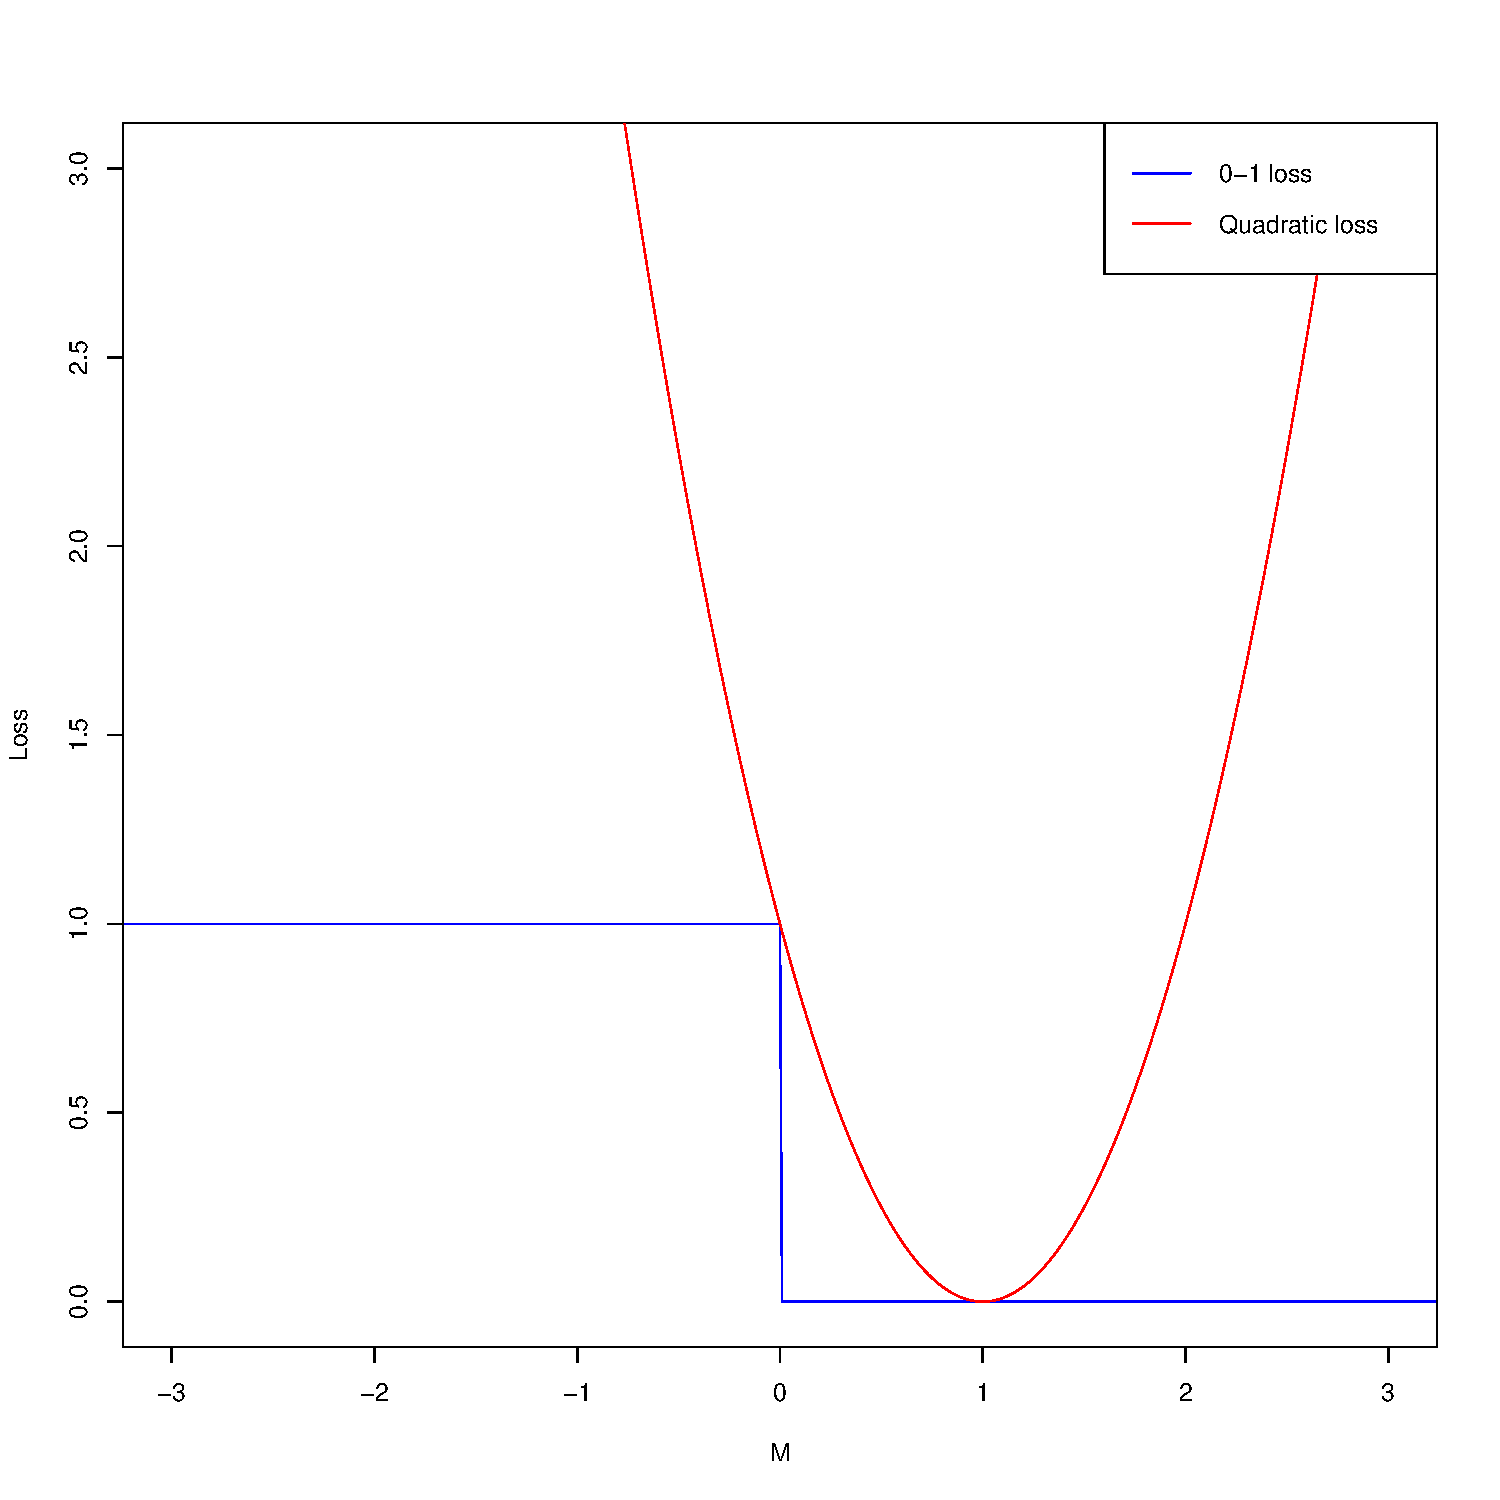
\includegraphics[width=0.8\linewidth]{quadraticLoss.pdf}
\end{center}
  \caption{Аппроксимация функции потерь}
  \label{fig:quadraticLoss}
\end{figure}

\section{Логистическая регрессия}
Рассмотрим логистическую регрессию как еще один метод построения байесовского классификатора.

Модель задается системой
\begin{align*}
  \log\frac{P(\eta = G_i \mid \boldsymbol{\xi} = \mathbf{x})}{P(\eta = G_K \mid \boldsymbol{\xi} = \mathbf{x})} = \beta_{i0} + \beta_{i}^\mathrm{T}\mathbf{x}, \quad i = 1,\ldots, K - 1.
\end{align*}
То есть задается $K-1$ log-odds или logit преобразованиями. Заметим, что в знаменателе можно поставить любой класс и оценки вероятностей не поменяются, то есть выбор класса в знаменателе случаен.

Если мы перейдем от логитов к вероятностям, то их сумма будет равна единице
\begin{align*}
  P(\eta = G_i \mid \boldsymbol{\xi} = \mathbf{x}) &= \frac{e^{\beta_{i0} + \beta^\mathrm{T}_i \mathbf{x}}}{1 + \sum_{k = 1}^{K - 1}e^{\beta_{k0} + \beta^\mathrm{T}_k \mathbf{x}}}, \quad i = 1,\ldots, K - 1,\\
  P(\eta = G_K \mid \boldsymbol{\xi} = \mathbf{x}) &= \frac{1}{1 + \sum_{k = 1}^{K - 1}e^{\beta_{k0} + \beta^\mathrm{T}_k \mathbf{x}}}.
\end{align*}

\subsection{Метод максимального правдоподобия и алгоритм Ньютона-Рафсона}
Для оценки параметров воспользуемся методом максимального правдоподобия. Рассмотрим логарифм функции максимального правдоподобия
\begin{align*}
  \ell(\theta) = \sum_{i = 1}^{N} \log P(\eta = G_k \mid \boldsymbol{\xi} = \mathbf{x}_i; \theta), \quad \theta = (\beta_{10}, \beta_{1}^\mathrm{T},\ldots,\beta_{(K-1)0}, \beta_{K - 1}^\mathrm{T}).
\end{align*}

Подробно обсудим случай двух классов $\mathcal{G} = \{0, 1\}$. Обозначим $p(\mathbf{x}, \theta) = P(\eta = 0 \mid \boldsymbol{\xi} = \mathbf{x}; \theta)$ и $1 - p(\mathbf{x}, \theta) = P(\eta = 1 \mid \boldsymbol{\xi} = \mathbf{x}; \theta)$. Тогда логарифм правдоподобия
\begin{align*}
  \ell(\beta) = \sum_{i = 1}^{N}(y_i\beta^\mathrm{T}\mathbf{x}_i - \log(1 + e^{\beta^\mathrm{T}\mathbf{x}_i})), \quad \beta = \{\beta_{10}, \beta_1\}.
\end{align*}

Чтобы максимизировать логарифм правдоподобия, приравниваем производные к нулю, получаем систему из $p + 1$ уравнения
\begin{align*}
  \frac{\partial \ell(\beta)}{\partial \beta} = \sum_{i = 1}^N \mathbf{x}_i (y_i - p(\mathbf{x}_i; \beta)) = 0.
\end{align*}

Для решения этой системы используем алгоритм Ньютона-Рафсона. Для начала выпишем гессиан логарифма правдоподобия
\begin{align*}
  \frac{\partial^2 \ell(\beta)}{\partial \beta \partial \beta^{\mathrm{T}}} = -\sum_{i = 1}^N x_ix_i^\mathrm{T} p(\mathbf{x}_i; \beta)(1 - p(\mathbf{x}_i; \beta)) = 0.
\end{align*}
Пусть $\beta^{old}$ -- некоторое начальное приближение вектора коэффициентов $\beta$, на каждой итерации он уточняется следующим образом:
\begin{align*}
  \beta^{new} = \beta^{old} - \left(\frac{\partial^2 \ell(\beta)}{\partial \beta \partial \beta^{\mathrm{T}}}\right)^{-1}\frac{\partial \ell(\beta)}{\partial \beta},
\end{align*}
где производные вычисляются в точке $\beta^{old}$.

Перейдем к матричным обозначениям. Обозначим $\mathbf{y}$ ответы $y_i$, $\mathbf{X}$ -- матрицу данных, $\mathbf{p} = (p(x_i; \beta^{old}))$, $\mathbf{W}$ -- диагональная матрица размером $N\times N$ весов, где $i$й элемент имеет вид $p(x_i;\beta^{old})(1 - p(x_i; \beta^{old}))$. Тогда
\begin{align*}
    \frac{\partial \ell(\beta)}{\partial \beta} &= \mathbf{X}^\mathrm{T}(\mathbf{y} - \mathbf{p})\\
    \frac{\partial^2 \ell(\beta)}{\partial \beta \partial \beta^{\mathrm{T}}} &= -\mathbf{X}^\mathrm{T}\mathbf{W}\mathbf{X}.
\end{align*}
Перепишем шаг алгоритма Ньютона-Рафсона
\begin{multline*}
  \beta^{new} = \beta^{old} + (\mathbf{X}^\mathrm{T}\mathbf{W}\mathbf{X})^{-1}\mathbf{X}^\mathrm{T}(\mathbf{y} - \mathbf{p}) = \\
  = (\mathbf{X}^\mathrm{T}\mathbf{W}\mathbf{X})^{-1}\mathbf{X}^\mathrm{T}\mathbf{W} (\mathbf{X}\beta^{old} + \mathbf{W}^{-1}(\mathbf{y} - \mathbf{p})) = \\
  = (\mathbf{X}^\mathrm{T}\mathbf{W}\mathbf{X})^{-1}\mathbf{X}^\mathrm{T}\mathbf{W}\mathbf{z}.
\end{multline*}
Мы переписали итерацию алгоритма как взвешенную регрессию, где в качестве ответа выступает вектор
\begin{align*}
  \mathbf{z} = \mathbf{X}\beta^{old} + \mathbf{W}^{-1}(\mathbf{y} - \mathbf{p}).
\end{align*}
На каждом шаге $\mathbf{p}$ меняется, а вместе с ним и $\mathbf{W}$, $\mathbf{z}$. Этот алгоритм называется iteratively reweighted least squares (IRLS) так как на каждом шаге решается задача
\begin{align*}
  \beta^{new} = \argmin_\beta (\mathbf{z} - \mathbf{X}\beta)^\mathrm{T} \mathbf{W}(\mathbf{z} - \mathbf{X}\beta).
\end{align*}

В качестве начального приближения $\beta^{old}$ можно взять оценки, полученные с помощью обычной линейной регрессии или просто $\beta^{old} = 0$. Сходимость нам не гарантируется, но обычно алгоритм сходится так как логарифм правдоподобия вогнутый.

\subsection{Минимизация эмпирического риска}
В логистической регрессии минимизируется аппроксимация:
  \begin{align*}
     Q(\beta) = \sum_{i = 1}^N \log(1 + e^{-y_i\beta^\mathrm{T}x_i}) \rightarrow \min_\beta,
  \end{align*}
то есть функция потерь имеет вид $\mathcal{L}(M_i(\beta)) = \log(1 + e^{-y_i\beta^\mathrm{T}x_i})$ (см. Рис. \ref{fig:LogLoss}).

\begin{figure}[h]
  \begin{center}
  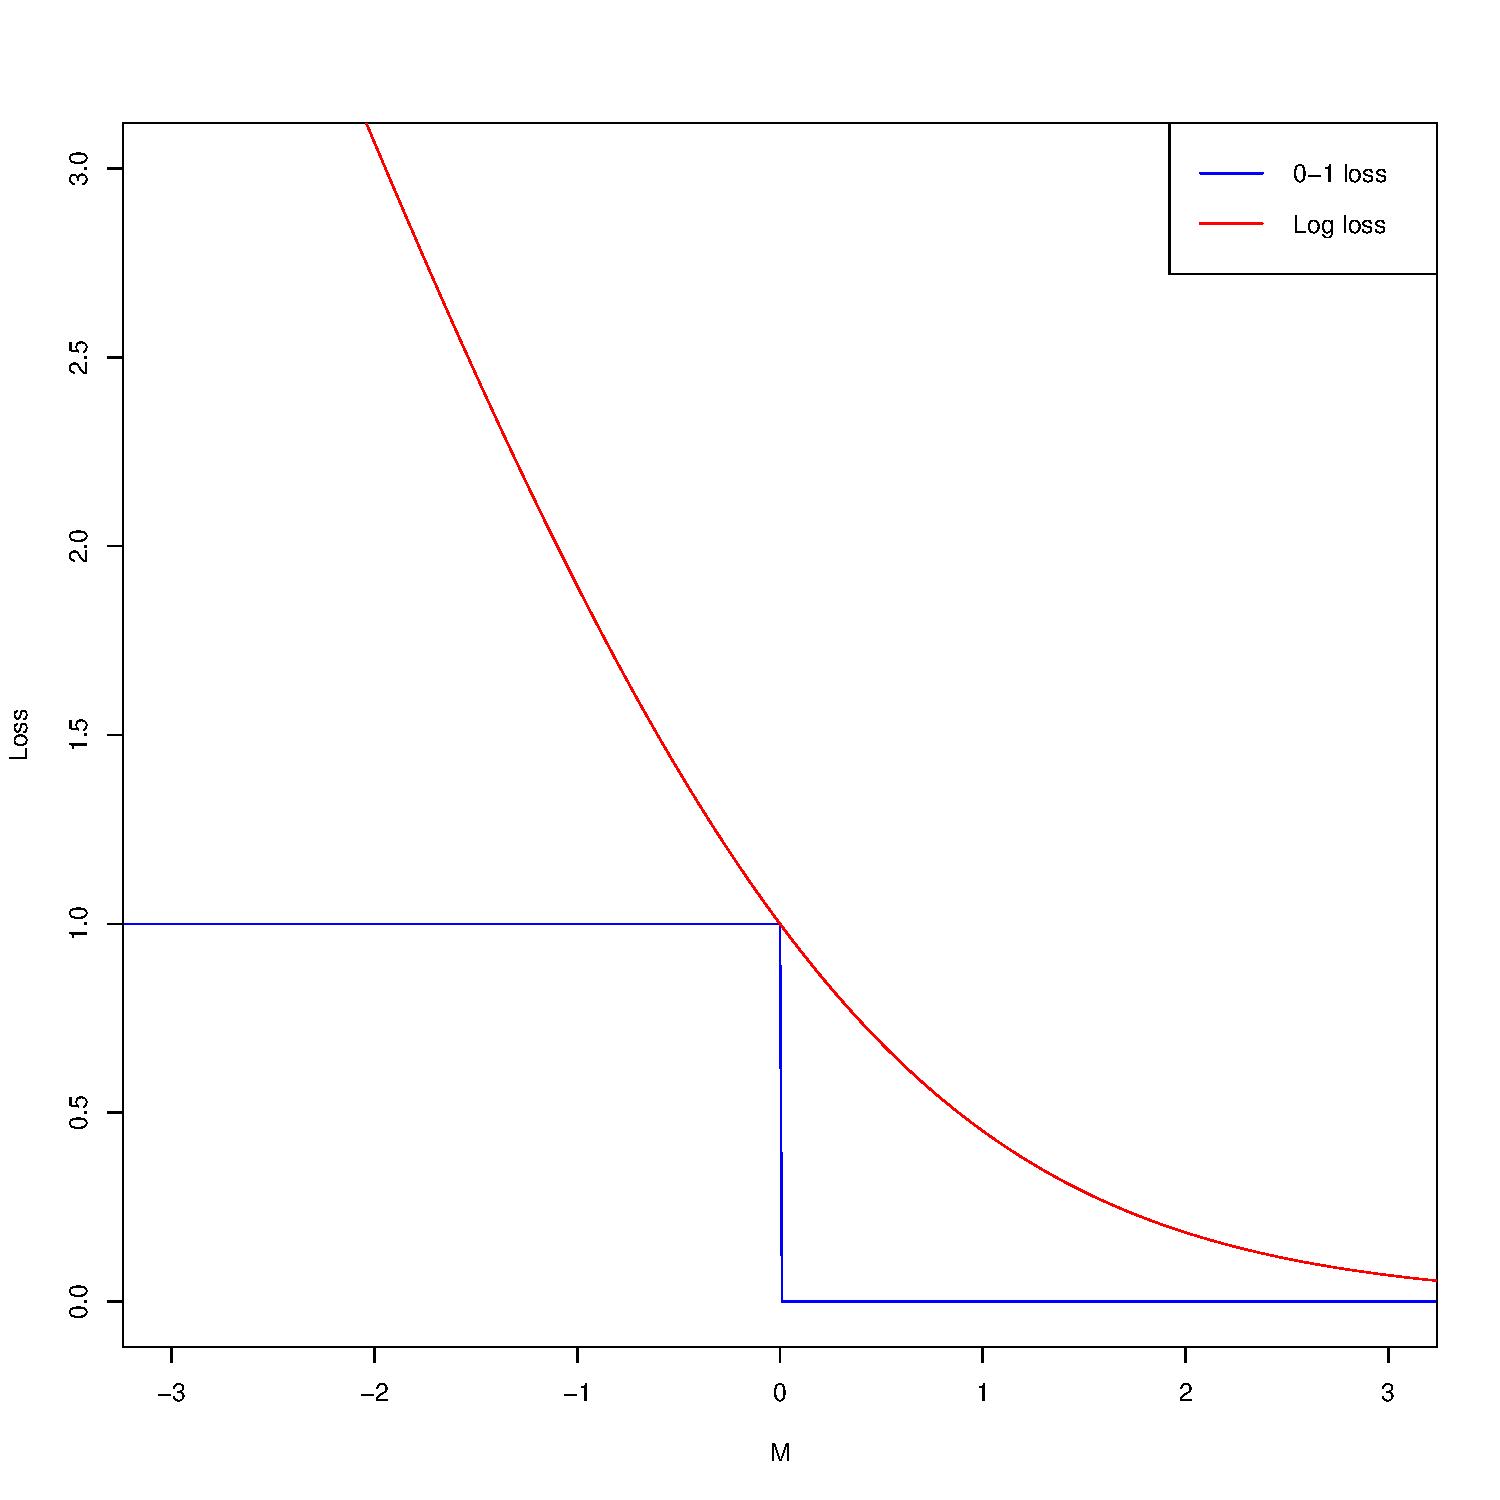
\includegraphics[width=0.8\linewidth]{LogLoss.pdf}
\end{center}
  \caption{Аппроксимация функции потерь}
  \label{fig:LogLoss}
\end{figure}

\subsection{Регуляризация}
Аналогично обычной линейной регрессии, можно отбирать признаки (осуществлять feature selection) с помощью LASSO (L1) или аналога Ridge Regression (L2). Для этого максимизируем соответственно
\begin{align*}
  \max_{\beta_0, \beta} \sum\limits_{i = 1}^N \left( y_i(\beta_0 + \beta^\mathrm{T}\mathbf{x}_i) - \log (1 + e^{\beta_0 + \beta^\mathrm{T}\mathbf{x_i}})\right) - \lambda \sum\limits_{j = 1}^p |\beta_j|,
\end{align*}
\begin{align*}
\max_{\beta_0, \beta} \sum\limits_{i = 1}^N \left( y_i(\beta_0 + \beta^\mathrm{T}\mathbf{x}_i) - \log (1 + e^{\beta_0 + \beta^\mathrm{T}\mathbf{x_i}})\right) - \lambda \sum\limits_{j = 1}^p \beta_j^2.
\end{align*}

Для нахождения точки максимума можно снова использовать алгоритм Ньютона-Рафсона.

Для feature extraction можно воспользоваться например анализом главных компонент.

\section{Логистическая регрессия против линейного дискриминантного анализа}
В пункте про линейный дискриминантный анализ мы получили линейную по $\mathbf{x}$ дискриминантную функцию как следствие предположения о нормальном распределении групп и одинаковых ковариационных матрицах. Можно посмотреть на log-posterior odds между классами $i$ и $K$ (или, что то же самое, на разделяющую их гиперплоскость) и получить
\begin{multline*}
  \log \frac{P(\eta = G_i \mid \boldsymbol{\xi} = \mathbf{x})}{P(\eta = G_K \mid \boldsymbol{\xi} = \mathbf{x})} = \\ = -\frac{1}{2} (\mu_i - \mu_K)^\mathrm{T} \Sigma^{-1}(\mu_i + \mu_K) + (\mu_i - \mu_K)^\mathrm{T} \Sigma^{-1}x + \log(\pi_i/\pi_K) = \\
  = \alpha_{i0} + \alpha_i^\mathrm{T}\mathbf{x}.
\end{multline*}
С другой стороны, линейная логистическая регрессия имеет линейные логиты по построению
\begin{align*}
  \log \frac{P(\eta = G_i \mid \boldsymbol{\xi} = \mathbf{x})}{P(\eta = G_K \mid \boldsymbol{\xi} = \mathbf{x})} = \beta_{i0} + \beta_i^\mathrm{T}\mathbf{x}.
\end{align*}
Модели выглядят очень похоже. Различие заключается в том как оцениваются линейные коэффициенты. Логистическая регрессия -- более общий подход, мы делаем меньше предположений.

Выпишем совместную плотность $X$ и $G$
\begin{align*}
  P(\boldsymbol{\xi} = \mathbf{x}, \eta = G_i) = P(\mathbf{x})P(\eta = G_i \mid \boldsymbol{\xi} = \mathbf{x}).
\end{align*}
И в линейном дискриминантном анализе, и в логистической регрессии второй множитель выражается как
\begin{align*}
  P(\eta = G_i \mid \boldsymbol{\xi} = \mathbf{x}) = \frac{e^{\beta_{i0} + \beta^\mathrm{T}_i \mathbf{x}}}{1 + \sum_{k = 1}^{K - 1}e^{\beta_{k0} + \beta^\mathrm{T}_k \mathbf{x}}}.
\end{align*}
В логистической регрессии $P(X)$ -- произвольная плотность, а параметры $P(G \mid X)$ оцениваются максимизацией условного правдоподобия (сумму логарифмов условных плотностей классов). Такой подход называют discriminative learning. Решается задача
\begin{align*}
  \ell(\theta) = \sum_{i = 1}^{N} \log P(\eta = y_i \mid \boldsymbol{\xi} = \mathbf{x}_i; \theta) \rightarrow \max_\theta.
\end{align*}

 С другой стороны, в LDA мы максимизируем полноценный логарифм функции правдоподобия совместной плотности
 \begin{align*}
   P(\mathbf{x} , \eta = G_i) =  \phi(\mathbf{x}; \mu_i, \Sigma)\pi_i,
 \end{align*}
где $\phi(\mathbf{x}; \mu_i, \Sigma)$  -- плотность нормального распределения. Такой подоход называют generative learning. Решается задача
\begin{align*}
  \ell(\mu_i, \Sigma) = \sum_{i = 1}^{N} \phi(\mathbf{x}_i; \mu_i, \Sigma)\pi_i \rightarrow \max_{\mu_i, \Sigma}.
\end{align*}

Оценив параметры нормального распределения, мы можем подставить их в выражения для логитов. В отличие от логистической регресси, плотность $P(X)$ здесь играет роль. Это смесь распределений
\begin{align*}
  P(\mathbf{x}) =  \sum_{i = 1}^K \phi(\mathbf{x}; \mu_i, \Sigma)\pi_i.
\end{align*}

Возникает вопрос, что нам дает такая модель? Предположение о нормальности распределения дает нам больше информации о параметрах, отсюда меньше дисперсия оценок. С другой стороны, точки, которые находятся далеко от разделяющей плоскости (у которых в логистической регрессии вес будет меньше), влияют на оценку ковариационной матрицы. Это значит, что LDA не является робастным по отношению к выбросам.

В логистической регрессии модель более гибкая, так как у нас меньше ограничений на распределения групп. Отсюда и меньшее количество параметров, которое необходимо оценивать.

Сравнить два подхода можно и с точки зрения минимизации эмпирического риска в терминах ML. Сразу становится ясно, что логистическая регрессия и линейный дискриминантный анализ решают разные задачи так как минимизируют разные аппроксимации эмпирического риска.

\section{Непараметрическое оценивание плотностей}
Выше мы строили байесовский классификатор исходя из каких-то модельных предположений. Ниже предложен непараметрический способ оценки плотностей.

Локальная непараметрическая оценка Парзена-Розенблата имеет следующий вид:
\begin{align*}
   \widehat{p}_h(\mathbf{z}) = \frac{1}{N}\sum_{i = 1}^N \prod_{j = 1}^p \frac{1}{h_j}K \left(\frac{z_j - x_{ij}}{h_j}\right),
\end{align*}
где $K(x)$ -- четная и нормированная функция $\int K(x) dx = 1$, которую называют ядром; $h > 0$ -- ширина окна, которая выбирается с помощью скользящего контроля (LOO).

Если $K(x)$ -- непрерывно, $\int K(x)^2 dx < \infty$ и найдется последовательность $h_N$ такая, что $\lim\limits_{N \rightarrow \infty}h_N = 0$ и $\lim\limits_{N \rightarrow \infty} Nh_N = \infty$, тогда $\widehat{p}_{h_m}(\mathbf{z}) \rightarrow p(x)$ п.в. при $N \rightarrow \infty$.

Метод парзеновского окна расширяется на случай произвольной метрики, а также на случай переменной ширины окна. Последнее помогает избежать проблему локальных сгущений в случае сильно неравномерного распределения. Одно и то же значение $h$ приведет к чрезмерному сглаживанию плотности в одних областях пространства и недостаточному в других.

Выбор ядра не влияет на качество оценки, но определяет гладкость функции $\widehat{p}_{h}$ и влияет на эффективность вычислений.

\begin{figure}[h]
  \begin{center}
  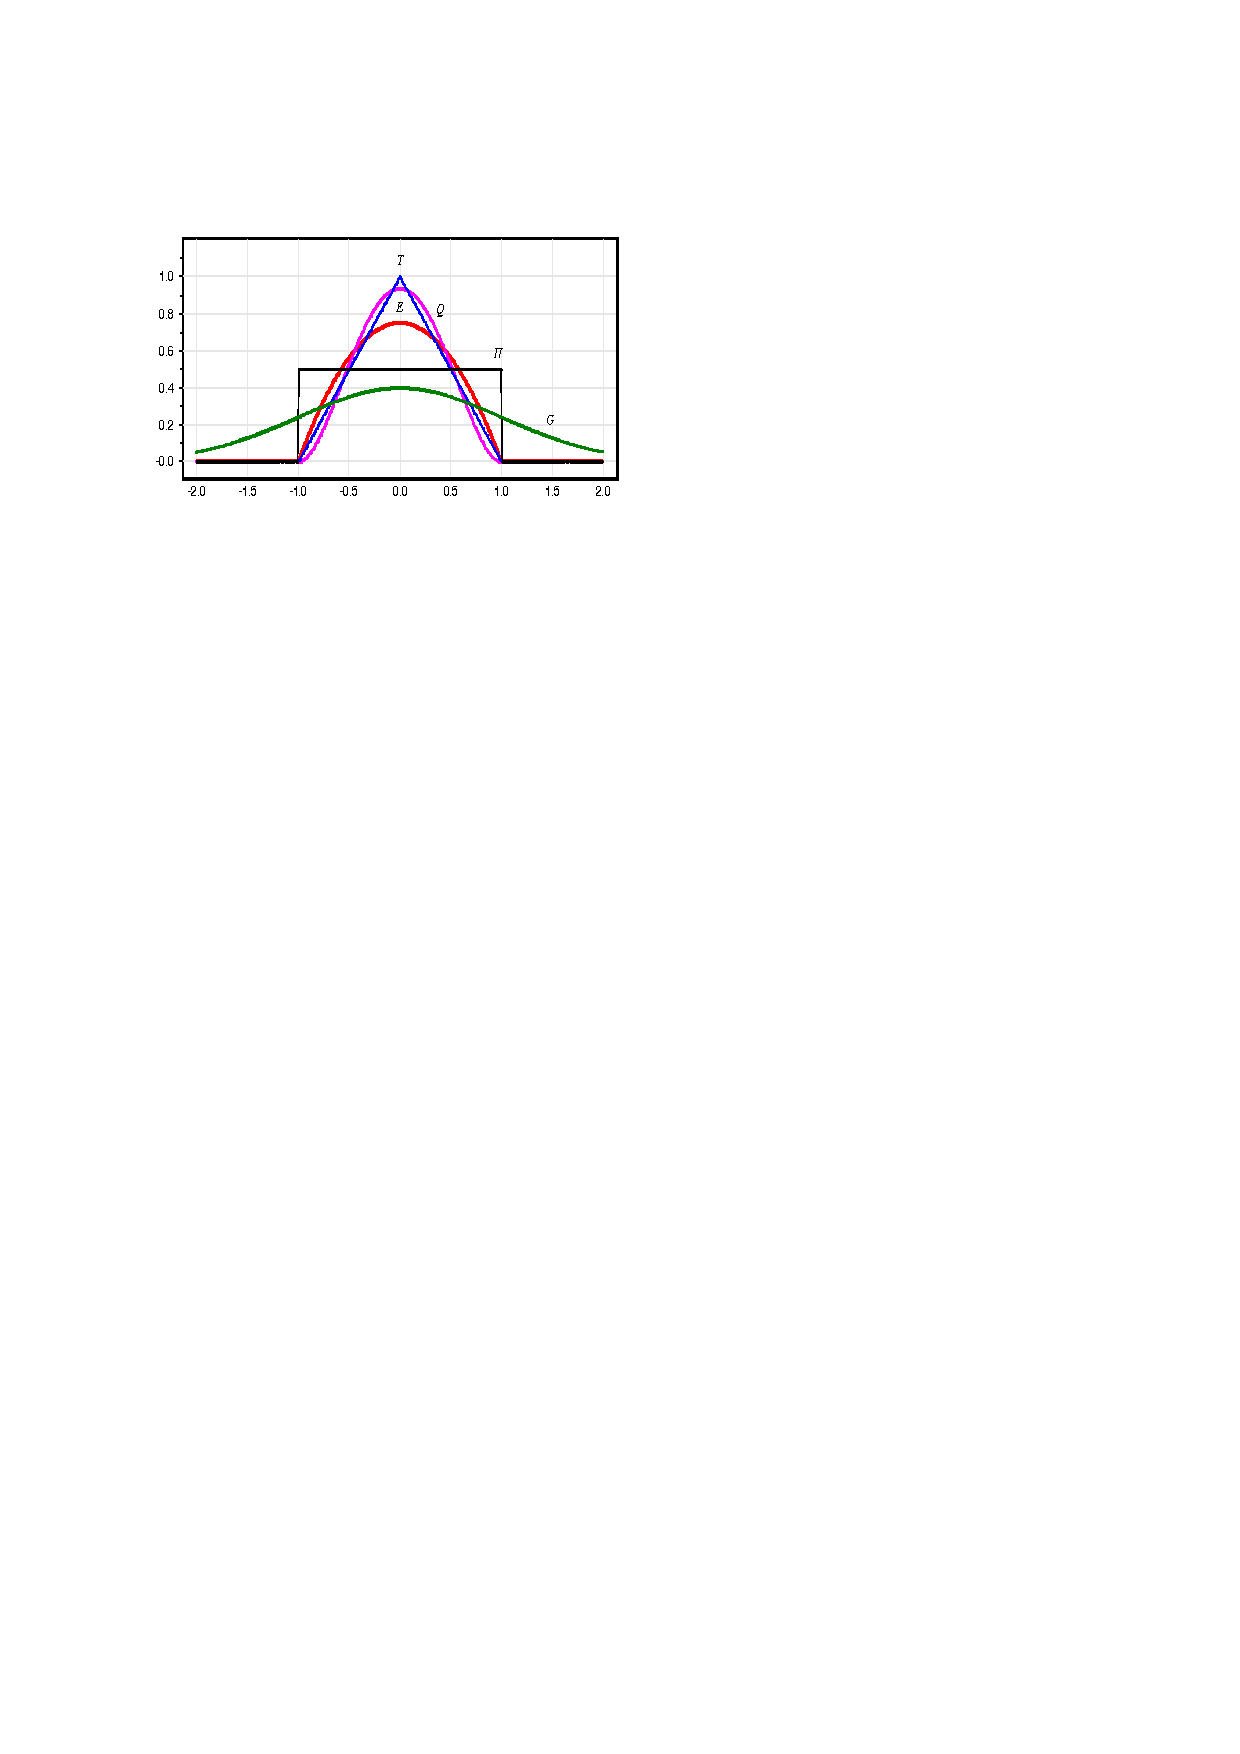
\includegraphics[width=0.8\linewidth]{kernels.pdf}
\end{center}
  \caption{Различные ядра: Е -- Епанечикова, Q -- Квартическое, Т -- Треугольное, G -- Гауссовское, П -- Прямоугольное}
  \label{fig:Kernels}
\end{figure}



\end{document}
